\section{Fourier's Physics Playground}

    \subsection{Maxwell's Electrodynamics}
    \frame{\sectionpage}

    \begin{frame}{In the beggining, God said:}
        \begin{equation*}
            \left\lbrace
            \begin{aligned}
                &\div{\vb{E}} = \frac{\rho}{\e}\\
                &\div{\vb{B}} = 0\\
                &\curl{\vb{E}} = - \pdv{\vb{B}}{t}\\
                &\curl{\vb{B}} = \m\vb{J}
 + \m\e\pdv{\vb{E}}{t}                        
            \end{aligned}
            \right.
        \end{equation*}
        
        \uncover<2>{and there was light!}
    \end{frame}
    
    \begin{frame}{Too hard, let's try something different}
        \begin{equation*}
            \left\lbrace
            \begin{aligned}
                &\vb{E} = - \grad{V} - \pdv{\vb{A}}{t} \\
                &\vb{B} = \curl{\vb{A}}
            \end{aligned}
            \right.
        \end{equation*}
    \end{frame}
    
    \begin{frame}{Wave Equations}
        \begin{equation*}
            \left\lbrace
            \begin{aligned}
                &\laplacian{V} - \frac{1}{c^2}\pdv[2]{V}{t} = - \frac{\rho}{\e}\\
                &\laplacian{\vb{A}} - \frac{1}{c^2}\pdv[2]{\vb{A}}{t} = - \m\vb{J}
            \end{aligned}
            \right.
        \end{equation*}
    \end{frame}
    
    \begin{frame}{All Wave Equations In One}
        \begin{equation*}
            \laplacian{\psi(\vb{r},t)} - \frac{1}{c^2}\pdv[2]{\psi}{t} (\vb{r},t) = - g(\vb{r},t)
        \end{equation*}
    \end{frame}
    
    \begin{frame}{Fourier's Opinion}
        \begin{equation*}
            \widehat{g}(\vb{r},\omega) = \frac{1}{\sqrt{2\pi}} \int_{-\infty}^{+\infty} g(\vb{r},t) e^{-i\omega t} \dd{t}
        \end{equation*}
        
        \begin{equation*}
            g(\vb{r},t) = \frac{1}{\sqrt{2\pi}} \int_{-\infty}^{+\infty} \widehat{g}(\vb{r},\omega) e^{i\omega t} \dd{\omega}
        \end{equation*}
    \end{frame}
    
    \begin{frame}{Fourier's Opinion}
        \begin{equation*}
            \widehat{\psi}(\vb{r},\omega) = \frac{1}{\sqrt{2\pi}} \int_{-\infty}^{+\infty} \psi(\vb{r},t) e^{-i\omega t} \dd{t}
        \end{equation*}
        
        \begin{equation*}
            \psi(\vb{r},t) = \frac{1}{\sqrt{2\pi}} \int_{-\infty}^{+\infty} \widehat{\psi}(\vb{r},\omega) e^{i\omega t} \dd{\omega}
        \end{equation*}
    \end{frame}
    
    \begin{frame}{Fourier's Opinion}
        \begin{equation*}
            \laplacian{\psi(\vb{r},t)} - \frac{1}{c^2}\pdv[2]{\psi}{t} (\vb{r},t) = - g(\vb{r},t)
        \end{equation*}
        
        \begin{equation*}
            \laplacian{\widehat{\psi}(\vb{r},\omega)} + \frac{\omega^2}{c^2} \widehat{\psi}(\vb{r},\omega) = - \widehat{g}(\vb{r},\omega)
        \end{equation*}
    \end{frame}
    
    \begin{frame}{Green Function}
        \uncover<+->{\begin{equation*}
            L \phi(\vb{r}) = - s(\vb{r})
        \end{equation*}}
        
        \uncover<+->{\begin{equation*}
            L G(\vb{r} - \vb{r'}) = - \dirac{\vb{r} - \vb{r'}}
        \end{equation*}}
        
        \uncover<+->{\begin{equation*}
            \phi(\vb{r}) = \int G(\vb{r} - \vb{r'}) s(\vb{r'}) \dd{\tau'}
        \end{equation*}}
        
        \uncover<+->{\begin{equation*}
            L \phi(\vb{r}) = \int L G(\vb{r} - \vb{r'}) s(\vb{r'}) \dd{\tau'} =  - \int \dirac{\vb{r} - \vb{r'}} s(\vb{r'}) \dd{\tau'} = -s(\vb{r})
        \end{equation*}}
    \end{frame}
    
    \begin{frame}{One At a Time}
        \uncover<+->{\begin{equation*}
            \laplacian{\widehat{\psi}(\vb{r},\omega)} + \frac{\omega^2}{c^2} \widehat{\psi}(\vb{r},\omega) = - \widehat{g}(\vb{r},\omega)
        \end{equation*}}
        
        \uncover<+->{\begin{equation*}
            \laplacian{G(\vb{r} - \vb{r'})} + \frac{\omega^2}{c^2} G(\vb{r} - \vb{r'}) = - \dirac{\vb{r} - \vb{r'}}
        \end{equation*}}
    \end{frame}
    
    \begin{frame}{Solution for $\vb{r} - \vb{r'} \neq \vb{0}$}
        \uncover<+->{\begin{equation*}
            \frac{1}{r}\dv[2]{(rG)}{r} + k^2 G = 0
        \end{equation*}}
        
        \uncover<+->{\begin{equation*}
            G(r) = \frac{A}{r}e^{\pm i k r}
        \end{equation*}}
    \end{frame}
    
    \begin{frame}{Recovering $0$ Psychological Trauma}
        \uncover<+->{\begin{equation*}
            \laplacian{G(\vb{r} - \vb{r'})} + \frac{\omega^2}{c^2} G(\vb{r} - \vb{r'}) = - \dirac{\vb{r} - \vb{r'}}
        \end{equation*}}
        
        \uncover<+->{\begin{equation*}
            A \int \laplacian{\frac{1}{r}} \dd{\tau'} + 4\pi A \frac{\omega^2}{c^2} \int \frac{r^2}{r} \dd{r}  = - \int \dirac{\vb{r} - \vb{r'}} \dd{\tau'}
        \end{equation*}}
        
        \uncover<+->{\begin{equation*}
            - 4 \pi A  = - 1
        \end{equation*}}
    \end{frame}
    
    \begin{frame}{Back To Our Problem}
        \uncover<+->{\begin{equation*}
            \widehat{\psi}(\vb{r}, \omega) = \int G(\rc)\widehat{g}(\vb{r'}, \omega) \dd{\tau'}
        \end{equation*}}
        
        \uncover<+->{\begin{equation*}
            G(\rc) = \frac{1}{4\pi \rc}e^{\pm i k \rc}
        \end{equation*}}
        
        \uncover<+->{\begin{equation*}
            \widehat{\psi}(\vb{r}, \omega) = \frac{1}{4\pi} \int \frac{\widehat{g}(\vb{r'}, \omega) e^{\pm i k \rc}}{\rc} \dd{\tau'}
        \end{equation*}}
    \end{frame}
    
    \begin{frame}{Actually Solving Our Problem}
        \uncover<+->{\begin{equation*}
            \psi(\vb{r},t) = \frac{1}{\sqrt{2\pi}} \int_{-\infty}^{+\infty} \widehat{\psi}(\vb{r},\omega) e^{i\omega t} \dd{\omega}
        \end{equation*}}
            
        \uncover<+->{\begin{equation*}
            \psi(\vb{r},t) = \frac{1}{4 \pi \sqrt{2\pi}} \iint \frac{\widehat{g}(\vb{r'}, \omega) e^{i \omega t \pm i \omega \frac{\rc}{c}}}{\rc} \dd{\omega} \dd{\tau'}
        \end{equation*}}
    \end{frame}
    
    \begin{frame}{Actually Solving Our Problem}
        \uncover<+->{\begin{equation*}
            \psi(\vb{r},t) = \frac{1}{4 \pi \sqrt{2\pi}} \iint \frac{\widehat{g}(\vb{r'}, \omega) e^{i \omega \prnt{t \pm \frac{\rc}{c}}}}{\rc} \dd{\omega} \dd{\tau'}
        \end{equation*}}
        
        \uncover<+->{\only<-2>{\begin{equation*}
            \psi(\vb{r},t) = \frac{1}{4 \pi} \int \frac{g(\vb{r'}, t \pm \frac{\rc}{c})}{\rc} \dd{\tau'}
        \end{equation*}}
        
        \only<3>{\begin{equation*}
            \psi(\vb{r},t) = \frac{1}{4 \pi} \int \frac{g(\vb{r'}, t - \frac{\rc}{c})}{\rc} \dd{\tau'}
        \end{equation*}}}
    \end{frame}
    
    \begin{frame}{Back at Maxwell's}
        \begin{equation*}
            V(\vb{r},t) = \frac{1}{4 \pi \e} \int \frac{\rho(\vb{r'}, t - \frac{\rc}{c})}{\rc} \dd{\tau'}
        \end{equation*}
        
        \begin{equation*}
            \vb{A}(\vb{r},t) = \frac{\m}{4 \pi} \int \frac{\vb{J}(\vb{r'}, t - \frac{\rc}{c})}{\rc} \dd{\tau'}
        \end{equation*}
    \end{frame}
    
    \begin{frame}{One Last Step} 
        \begin{equation*}
            \left\lbrace
            \begin{aligned}
                &\vb{E} = - \grad{V} - \pdv{\vb{A}}{t} \\
                &\vb{B} = \curl{\vb{A}}
            \end{aligned}
            \right.
        \end{equation*}
    \end{frame}
    
    \begin{frame}{Jefimenko Equations}
        \begin{equation*}
            \vb{E}(\vb{r},t) = \frac{1}{4\pi\e}\int \frac{\hrc}{\rc^2}\rtd{\rho} + \frac{\hrc}{c\rc} \rtd{\pdv{\rho}{t}} - \frac{1}{c^2\rc} \rtd{\pdv{\vb{J}}{t}} \dd{\tau'}
        \end{equation*}
                    
        \begin{equation*}
            \vb{B}(\vb{r},t) = \frac{\m}{4\pi}\int \prnt{\frac{1}{\rc^2} \rtd{\vb{J}} + \frac{1}{c\rc} \rtd{\pdv{\vb{J}}{t}}} \cp \hrc \dd{\tau'}
        \end{equation*}
    \end{frame}
    
    \subsection{Heisenberg's Uncertainty Principle}
    \frame{\sectionpage}
    \begin{frame}{Position and Momentum}
        \uncover<+->{\begin{equation*}
            \psi(x) = \bra{x}\ket{\psi} = \int \bra{x}\ket{k} \bra{k}\ket{\psi} \dd{k} = \frac{1}{\sqrt{2\pi}} \int e^{ikx} \psi(k) \dd{k}
        \end{equation*}}
        
        \uncover<+->{\begin{equation*}
            \psi(k) = \bra{k}\ket{\psi} = \int \bra{k}\ket{x} \bra{x}\ket{\psi} \dd{x} = \frac{1}{\sqrt{2\pi}} \int e^{-ikx} \psi(x) \dd{x}
        \end{equation*}}
    \end{frame}
    
    \begin{frame}{Position and Momentum (but weirder)}
        \uncover<+->{\begin{equation*}
            \left\lbrace
            \begin{aligned}
                &X\ket{\psi} = x \psi(x) \\
                &K \ket{\psi} = - i \pdv{\psi}{x} (x)
            \end{aligned}
            \right.
        \end{equation*}}
        
        \uncover<+->{\begin{equation*}
            \left\lbrace
            \begin{aligned}
                &X\ket{\psi} = - i \pdv{\psi}{k} (k) \\
                &K \ket{\psi} = k \psi(k)
            \end{aligned}
            \right.
        \end{equation*}}
    \end{frame}
    
    \begin{frame}{Fourier Diplomacy}
        \uncover<+->{\begin{equation*}
            \ket{x} \xleftrightarrow[\mathcal{F}^{-1}]{\mathcal{F}} \ket{k}
        \end{equation*}}
    \end{frame}
    
    \begin{frame}{Fourier Uncertainty}
        \begin{enumerate}
            \item<+-> $\psi(x):$ what is $x$?
            \item<+-> $\psi(k):$ what is $k$?
        \end{enumerate}
    \end{frame}
    
    \begin{frame}{Definite Position}
        \begin{equation*}
            \psi(x) = \sqrt{\frac{\pi}{2}}\prnt{\dirac{x-x_0} + \dirac{x+x_0}}    
        \end{equation*}
        
        \centering 
        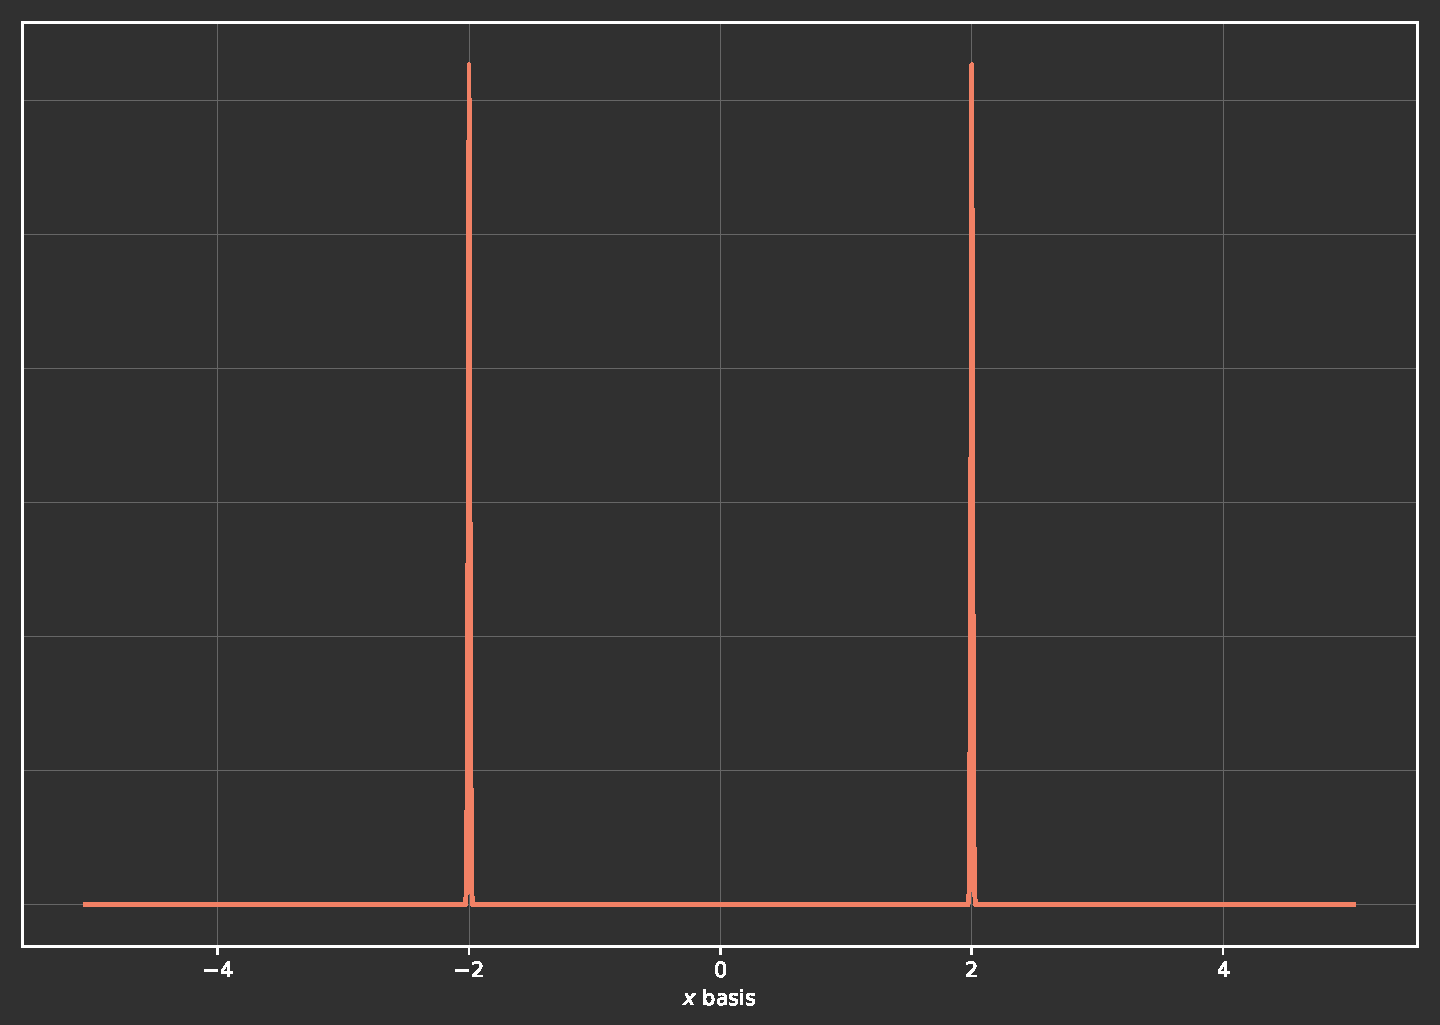
\includegraphics[height = 0.65 \textheight]{images/Pulse3-Fourier.pdf}
    \end{frame}
    
    \begin{frame}{Undefinite Momentum}
        \begin{equation*}
            \psi(k) = \cos(x_0 k) 
        \end{equation*}
        
        \centering
        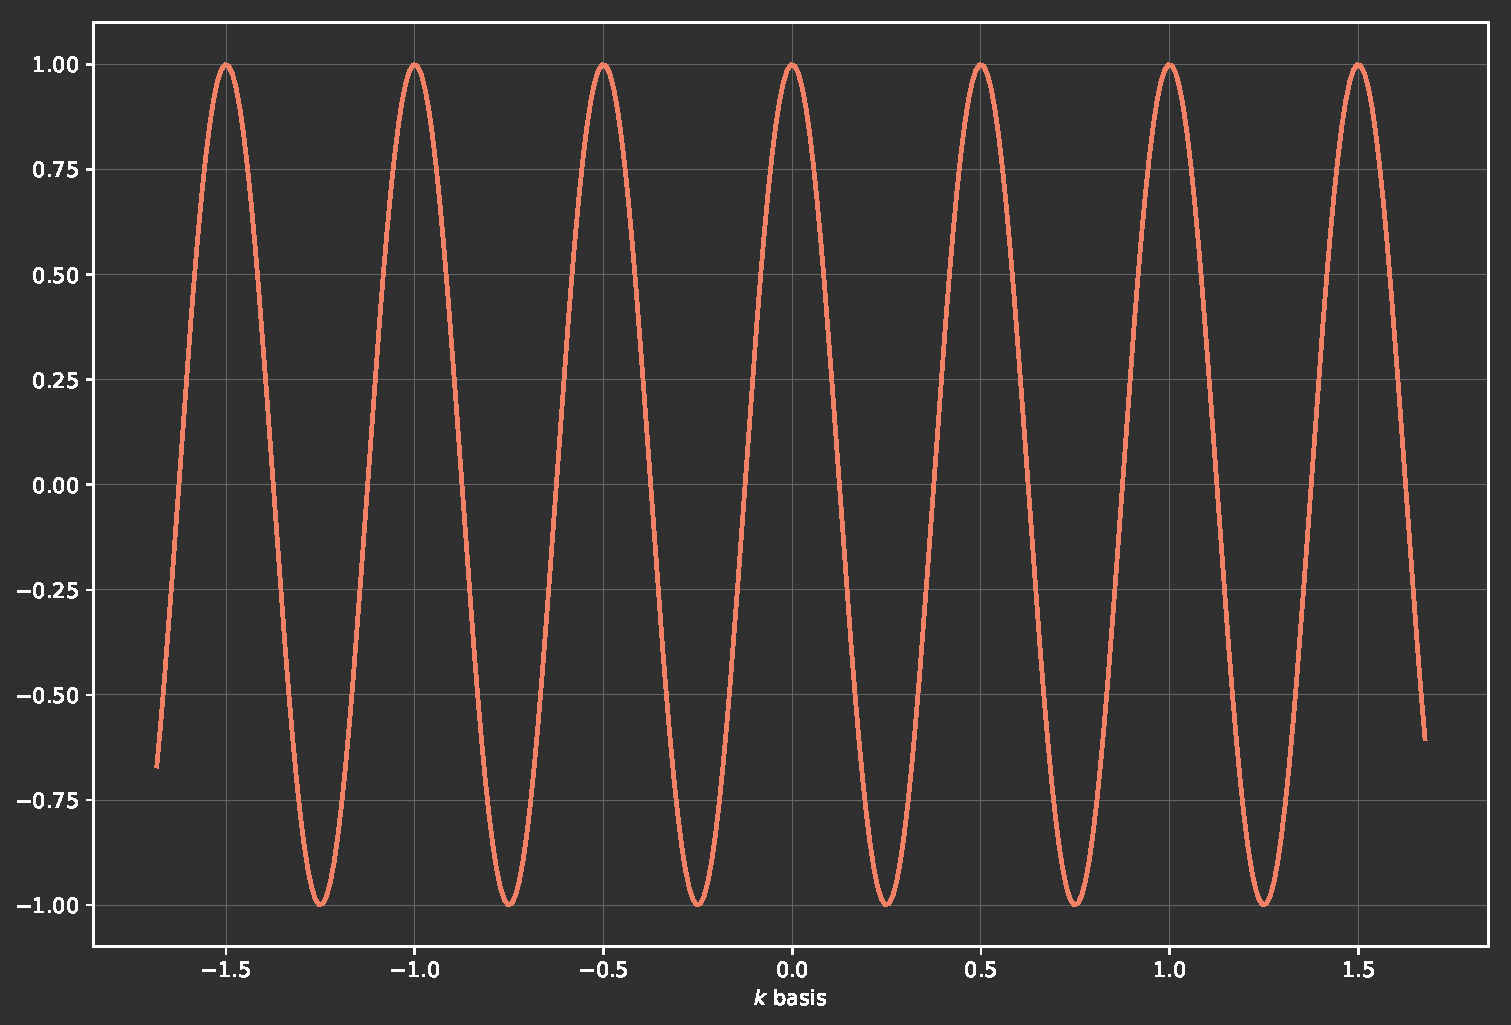
\includegraphics[height = 0.65 \textheight]{images/Pulse3.pdf}
    \end{frame}
    
    \begin{frame}{Uncertainty Relation}
        \begin{block}{\centering$\sigma_x\sigma_p \geq \frac{\hbar}{2}$}
            The uncertainty relation is a consequence of the general fact that anything narrow in one space is wide in the transform space and vice versa. So if you are a 45 kg weakling and are taunted by a 270 kg bully, just ask him to step into momentum space!
        
            \alert{Ramamurti Shankar}
        \end{block}
    \end{frame}